<<<<<<< HEAD
% kelompok Eratosthenes
% Boby Jamis Hari Sel (1154040)
% Diki Wahyu Nugraha (1154059)
% Restiyana Dwi Astuti (1154077)
% Rizki Abdi Perdana (1154007)
% Sabda Alamsyah (1154111)

\section{Eratosthenes}
Lebih dari 2000 tahun yang lalu Eratosthenes membandingkan posisi Matahari di dua lokasi untuk menentukan ukuran bumi dengan alasan yang akurat.
Berdasarkan \cite{plochmann1983dictionary} Eratosthenes lahir di Yunani pada koloni yang bernama Cyrene, sekarang disebut kota Shahhat, Libya, Sebagai pemuda, dia  pergi ke athena demi melanjutkan studinya. Lalu ua kembali ke Cyrene, dan membuat nama untuk dirinya sendiri untuk kebutuhan ilmiah sehingga penguasa Yunani di Mesir membawanya ke Aleksandria.
Seorang pria yang mempunyai banyak talenta, Eratosthenes adalah seorang pustakawan, geografer, matematikawan, astronom, sejarahwan dan penyair. Teman-temannya di perpustakaan menjulukinya sebagai Pentathlos atau atlit yang berkompetisi dalam lima acara yang berbeda. Julukan itu seperinya cocok ditujukan kepada untuk seorang penerima beasiswa dari banyak bidang studi. Banyak dari tulisan karya Eratosthenes telah hilang tetapi ada beberapa orang yang melaporkan pekerjaannya telah ditemukan. \cite{lasky2008librarian}
\begin{figure}[ht]
	\centerline{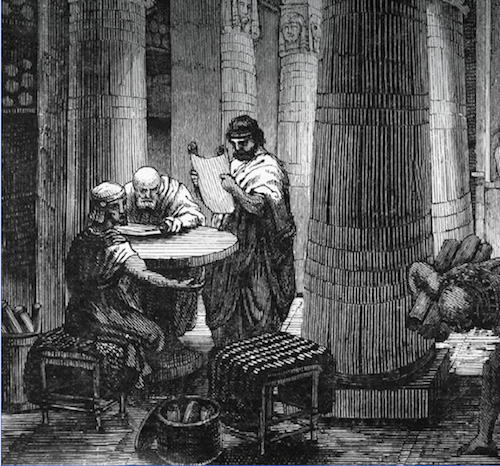
\includegraphics[width=1\textwidth]{figures/illustrasi.jpg}}
	\caption{ilustrasi yang tidak bertanggal dari para ilmuwan di Perpustakaan Alexandria © Bettmann / CORBIS}
	\label{illustrasi}
	\end{figure}
\subsection{Bapak Geografi}
Eratosthenes melanjutkan pengetahuannya tentang Bumi. Dengan menggunakan penemuan dan pengetahuan tentang ukuran dan bentuknya, dia mulai membuat sketsa. Di Perpustakaan Alexandria ia memiliki akses ke berbagai buku perjalanan, yang berisi berbagai bentuk informasi dan representasi dunia. \cite{smith2005dictionary} Dalam karya jilid tiga-nya Geografi (bahasa Yunani: Geographika), dia menggambarkan dan memetakan seluruh dunia yang dikenalnya, bahkan membagi Bumi menjadi lima zona iklim: \cite{grimbly2013encyclopedia} dua zona pembekuan di sekitar kutub, dua zona beriklim sedang, dan sebuah zona yang meliputi khatulistiwa dan daerah tropis. Ia telah menemukan geografi. Dia menciptakan terminologi yang masih digunakan sampai sekarang. Dia meletakkan grid garis tumpang tindih di atas permukaan Bumi. Dia menggunakan kesejajaran dan garis meridian untuk menghubungkan setiap tempat di dunia. Sekarang mungkin untuk memperkirakan jarak seseorang dari lokasi dasar jaringan ini di atas permukaan Bumi. Dalam Geografi nama-nama lebih dari 400 kota dan lokasi mereka ditunjukkan:  Sayangnya, Geografi-nya telah hilang dari sejarah, Pliny, Polybius, Strabo, dan Marcianus. \cite{roller2010eratosthenes}
Buku pertama adalah pengantar dan memberikan ulasan tentang pendahulunya, mengakui kontribusi mereka yang dia susun di perpustakaan. Dalam buku ini Eratosthenes mengecam Homer karena tidak memberikan wawasan tentang apa yang sekarang digambarkannya sebagai geografi. Ketidaksetujuannya terhadap topografi Homer membuat marah banyak orang yang percaya bahwa dunia digambarkan dalam Odyssey sebagai hal yang sah. \cite{eckerman2011eratosthenes} Bumi adalah dunia yang tak tergoyahkan; Sementara di permukaannya ada tempat yang sedang berubah. Dia telah berhipotesis bahwa pada suatu waktu Mediterania adalah danau besar yang menutupi negara-negara yang mengelilinginya; dan hanya terhubung ke barat saat sebuah lorong telah dibuka dalam sejarahnya.
Dalam buku kedua adalah penemuannya tentang keliling bumi. Di sinilah, menurut Pliny, ``Dunia digenggam.`` Eratosthenes menggambarkan kisah terkenalnya tentang sumur di Syene, yang dijelaskan di atas. Buku ini akan dianggap sebagai teks tentang geografi matematika.
Buku ketiganya tentang Geografi berisi geografi politik. Dia mengutip negara-negara dan menggunakan garis sejajar untuk membagi peta menjadi beberapa bagian, untuk memberikan deskripsi alam yang akurat. Ini adalah terobosan, dan bisa dianggap sebagai awal geografi. \cite{smith2005dictionary}
\subsection{Mempelajari Bumi}
Eratosthenes mungkin orang pertama yang menggunakan kata geografi. Dia menciptakan sistem garis bujur dan garis lintang dan membuat peta dari dunia yang sekarang dikenal. Dia juga merancang sistem untuk menemukan penomoran utama — bilangan bulat yang hanya dapat dibagi sendiri atau dengan angka 1. Metode ini, masih digunakan sampai hari ini.
Pada saat itu, Eratosthenes mengusulkan sebuah algoritma sederhana untuk menemukan bilangan prima. Algoritma ini dikenal dalam matematika sebagai ``Sieve of Eratosthenes.``
Dalam matematika, Sieve of Eratosthenes (Yunani: κόσκινον Ἐρατοσθένους), salah satu dari sejumlah saringan bilangan prima, adalah algoritma kuno yang sederhana untuk menemukan semua bilangan prima sampai batas tertentu. Hal itu terjadi karena secara iteratif menandai sebagai komposit, yaitu, tidak prima, kelipatan masing-masing prima, dimulai dengan kelipatan 2. Kelipatan bilangan prima yang diberikan dihasilkan mulai dari yang prima, sebagai urutan angka dengan perbedaan yang sama, sama dengan yang prima, antara angka berurutan. Ini adalah perbedaan kunci saringan dari penggunaan divisi percobaan untuk menguji secara berurutan setiap nomor kandidat untuk dibagi masing-masing prima.
Eeratosthenes juga yang pertama menghitung sumbu kemiringan bumi, yang dia pikir dengan tingkat akurasi yang tinggi; temuan dilaporkan oleh Ptolemy (85-165 M). Eratosthenes juga menghitung jarak dari bumi ke bulan dan ke matahari, tetapi dengan tingkat akurasi yang rendah. Ia membuat katalog 675 bintang. Ia membuat kalender dengan tahun kabisat dan meletakkan dasar chro- nology di dunia barat dengan penyelenggaraan tanggal sastra dan politik kegiatan dari pengepungan Troy (sekitar 1194 - 1184 SM) ke dalam waktu ia sendiri.
Namun, pencapaiannya yang paling abadi adalah perhitungan lingkar bumi yang sangat akurat (jarak di sekitar lingkaran atau bola). Dia menghitung ini dengan menggunakan geometri dan trigonometri sederhana dan dengan mengenali Bumi sebagai bola di ruang angkasa. Sebagian besar ilmuwan Yunani pada masa Aristoteles (384-322 SM) sepakat bahwa Bumi adalah sebuah bola, tapi tidak ada yang tahu seberapa besar itu.
Bagaimana para ilmuwan Yunani mengetahui bahwa bumi adalah sebuah lingkungan? Mereka mengamati bahwa kapal menghilang di atas cakrawala sementara tiang-tiang mereka masih terlihat. Mereka melihat bayangan melengkung Bumi di Bulan selama gerhana bulan. Dan mereka melihat perubahan posisi bintang di langit.
\begin{figure}[ht]
	\centerline{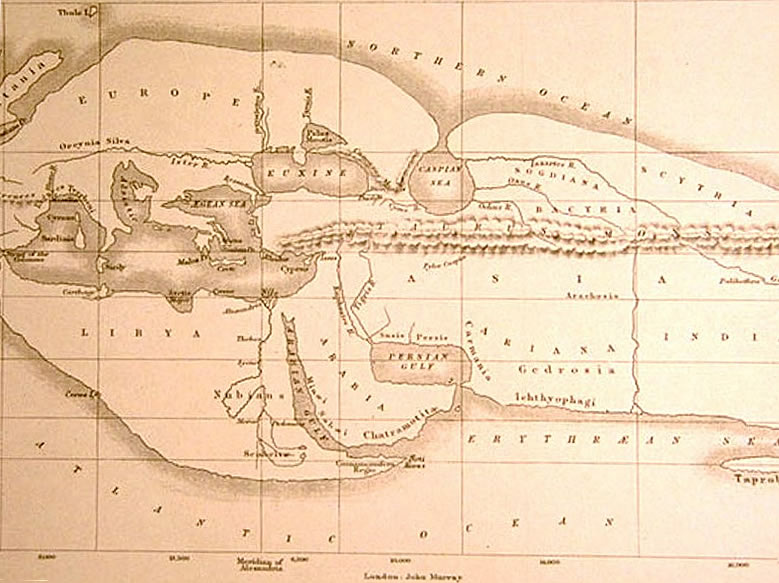
\includegraphics[width=1\textwidth]{figures/194BCEworldmap.jpg}}
	\caption{Rekonstruksi Eratosthenes c. 194 SM peta dunia, dari E.H. Bunbury's 1883 Sejarah Geografi Kuno di antara orang Yunani dan Romawi dari Abad Pertengahan sampai Kejatuhan Kekaisaran Romawi, ranah publik}
	\label{194BCEworldmap}
	\end{figure}
\subsection{Mengukur Bumi}
Eratosthenes mendengar tentang sumur terkenal di kota Swenet Mesir (Syene dalam bahasa Yunani, dan sekarang dikenal sebagai Aswan), di Sungai Nil. Siang hari satu hari setiap tahun - titik balik matahari musim panas (antara 20 Juni dan 22 Juni) - sinar matahari bersinar langsung ke dalam lubang dalam. Mereka hanya menyinari air di bagian bawah, bukan sisi sumur seperti pada hari-hari lain, membuktikan bahwa Matahari langsung di atas kepala. (Syene terletak sangat dekat dengan apa yang kita sebut Tropic of Cancer,  23,5 derajat ke utara, garis lintang paling utara di mana Matahari selalu berada di atas kepala pada siang hari.)
Eratosthenes mendirikan sebuah tiang di Alexandria, dan pada titik balik matahari musim panas ia mengamati bahwa ia melemparkan bayangan, membuktikan bahwa Matahari tidak berada di atas kepala tetapi sedikit ke selatan. Mengakui kelengkungan Bumi dan mengetahui jarak antara kedua kota memungkinkan Eratosthenes untuk menghitung lingkar planet.
\cite{nicastro2008circumference} Eratosthenes bisa mengukur sudut sinar matahari dari vertikal dengan membagi panjang kaki di seberang sudut (panjang bayangan) dengan kaki yang bersebelahan dengan sudut (tinggi tiang). Ini memberinya sudut 7,16 derajat. Dia tahu bahwa lingkar bumi membentuk lingkaran 360 derajat, jadi 7,12 (atau 7,2, untuk membagi 360 secara merata sampai 50) derajatnya kira-kira seper lima puluh keliling. Dia juga tahu perkiraan jarak antara Alexandria dan Syene, jadi dia bisa mengatur persamaan ini:

Eratosthenes memperkirakan jarak dari Alexandria ke Syene sebanyak 5.000 stadion, atau sekitar 500 mil (800 kilometer). Dia membuat estimasi ini dari saat dibutuhkan pejalan kaki, yang dilatih untuk mengukur jarak dengan mengambil langkah reguler, untuk berjalan-jalan di antara kota-kota. Dengan memecahkan persamaan tersebut, dia menghitung keliling 250.000 stadia, atau 25.000 mil (40.000 kilometer) seperti pada gambar \ref{diagrampengukuranbumi}.
\begin{figure}[ht]
	\centerline{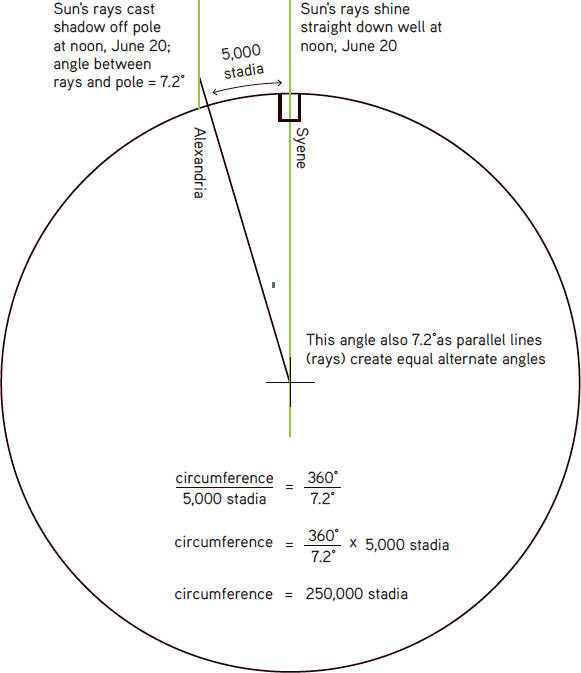
\includegraphics[width=1\textwidth]{figures/diagrampengukuranbumi.png}}
	\caption{Sebuah diagram yang menunjukkan bagaimana Eratosthenes mengukur Bumi, diakses dari Simon Fraser University Online}
	\label{diagrampengukuranbumi}
	\end{figure}
Beberapa sumber kesalahan merembet ke dalam perhitungan Eratosthenes dan interpretasi kita terhadapnya. Untuk satu hal, dia menggunakan unitnya untuk mengukur satuan "stadion" Yunani atau stadion atletik. Tapi tidak semua stadion dibangun dengan panjang yang sama. Di Yunani sebuah stadion setara dengan 185 meter (607 kaki), sedangkan di Mesir stadion berjarak sekitar 157,5 meter (517 kaki). Kami tidak tahu unit mana yang digunakan Eratosthenes. Jika dia menggunakan ukuran Yunani, perhitungannya akan turun sekitar 16 persen. Jika dia menggunakan orang Mesir, kesalahannya akan berada di bawah 2 persen dari lingkar bumi sebenarnya dari 24.860 mil (40.008 kilometer).
Satu abad setelah Eratosthenes, astronom Yunani Posidonius dari Rhodes (sekitar 135-51 SM) menghitung lingkar bumi. Posidonius menggunakan bintang Canopus sebagai kerangka acuan: ketika bintang tersebut terlihat di cakrawala di Rhodes, itu adalah 7,5 derajat di atas cakrawala di Alexandria. Perhitungan pertamanya hampir benar, tapi dia merevisi jarak antara Rhodes dan Alexandria, yang menghasilkan angka yang sebanding dengan sekitar 18.000 mil (sekitar 29.000 kilometer), sekitar 28 persen lebih kecil dari lingkar sebenarnya. Ptolemy melaporkan perhitungan Posidonius dan bukan kata-kata Eratosthenes, dan tulisan Ptolemy inilah yang menemukan jalan mereka menuju Christopher Columbus. Jika Ptolemy telah menggunakan sosok Eratosthenes yang lebih besar dan lebih akurat untuk keliling bumi, Columbus mungkin tidak akan pernah berlayar ke barat.
Eratosthenes hidup sampai usia 82 tahun, saat dia kelaparan sampai mati karena dia takut pada awitan kebutaan.
\subsection{Prestasi}
Eratosthenes digambarkan oleh Leksikon Suda sebagai Πένταθλος (Pentathlos) yang dapat diterjemahkan sebagai ``All-Rounder``, karena ia ahli dalam berbagai hal: Dia adalah seorang polymath sejati. Dia dijuluki Beta karena dia hebat dalam banyak hal dan mencoba mendapatkan setiap informasi, namun tidak pernah mencapai peringkat tertinggi dalam segala hal; Straboaccounts Eratosthenes sebagai matematikawan di antara ahli geografi dan ahli geografi di kalangan matematikawan.
\begin{itemize}
 
\item Eusebius dari Kaisarea dalam bukunya Preparatio Evangelica mencakup sebuah bab singkat dari tiga kalimat pada jarak selestial (Kitab XV, Bab 53). Dia menyatakan dengan sederhana bahwa Eratosthenes menemukan jarak ke Matahari untuk menjadi ``σταδίων μυριάδας τετρακοσίας καὶ ὀκτωκισμυρίας`` (secara harfiah 	``stadion miriad 400 dan 80.000``) dan jarak ke Bulan menjadi 780.000 stadion. Ungkapan jarak ke Matahari telah diterjemahkan sebagai 4.080.000 stadia (1903 terjemahan oleh E. H. Gifford), atau sebagai 804.000.000 stadia (edisi Edouard des Places, bertanggal 1974-1991). Artinya tergantung pada apakah Eusebius berarti 400 segudang ditambah 80.000 atau ``400 dan 80.000`` segudang. Dengan stadion 185 m, 804.000.000 stadion adalah 149.000.000 km, kira-kira jaraknya dari Bumi ke Matahari.
\item Menurut \cite{smith2005dictionary} Eratosthenes juga menghitung diameter Matahari. Menurut Macrobious, Eratosthenes membuat diameter Matahari menjadi sekitar 27 kali lipat dari Bumi. Angka sebenarnya kira-kira 109 kali.
\item Selama berada di Perpustakaan Alexandria, Eratosthenes merancang sebuah kalender dengan menggunakan ramalannya tentang ekliptika Bumi. Dia menghitung bahwa ada 365 hari dalam setahun dan setiap tahun keempat akan ada 366 hari.
\item Dia juga sangat bangga dengan solusinya untuk Menggandakan Cube. Motivanya adalah bahwa ia ingin menghasilkan ketapel. Eratosthenes membangun perangkat gambar garis mekanis untuk menghitung kubus, yang disebut mesolabio. Dia mendedikasikan solusinya untuk Raja Ptolemy, menyajikan sebuah model di perunggu dengan sebuah surat dan sebuah epigram. Archimedes adalah teman Eratosthenes dan dia juga mengerjakan alat perang dengan matematika. Archimedes mendedikasikan bukunya The Method to Eratosthenes, mengetahui cintanya untuk belajar dan matematika. \cite{chondros2010archimedes}
\end{itemize}
\subsection{Pekerjaan}
Eratosthenes adalah salah satu tokoh ilmiah paling terkemuka di masanya, dan menghasilkan karya-karya yang mencakup pengetahuan luas sebelum dan selama waktunya di Perpustakaan. Dia menulis banyak topik - geografi, matematika, filsafat, kronologi, kritik sastra, tatabahasa, puisi, dan bahkan komedi lama. Sayangnya, hanya ada sisa fragmen karya-karyanya setelah Penghancuran Perpustakaan Alexandria.
\subsection{Gelar}
\begin{enumerate}

\item	Platonikos
\item	Hermes
\item	Erigone
\item	Chronographies
\item	Pemenang Olimpiade
\item	 Περὶ τῆς ἀναμετρήσεως τῆς γῆς (Pada Pengukuran Bumi) (hilang, diringkas oleh Cleomedes) \cite{thomasselections}
\item	Гεωγραφικά (Geographika) (hilang, dikritik oleh Strabo)
\item	Arsinoe (sebuah memoar Ratu Arsinoe; hilang; \cite{gulickathenaeus})
\item	 Ariston (tentang Aristo dari Chios kecanduan kemewahan); kalah; dikutip oleh Athenaeus di Deipnosophistae) \cite{gulickathenaeus}
\item	Koleksi fragmen mitos Helenistik tentang rasi bintang, yang disebut Catasterismi (Katasterismoi), dikaitkan dengan Eratosthenes, mungkin untuk menambah kredibilitasnya.
\end{enumerate}
=======
% Kelompok 3
% Restiyana Dwi Astuti (1154077)
% Boby Jamis Hari Sel (1154040)
% Diki Wahyu Nugraha (1154059)
% Rizki Abdi Perdana (1154107)
% Sabda Alamsyah (1154111)

\section(Eratosthenes)
Lebih dari 2000 tahun yang lalu Eratosthenes membandingkan posisi Matahari di dua lokasi untuk menentukan ukuran bumi dengan alasan yang akurat.
Berdasarkan \cite{plochmann1983dictionary} Eratosthenes lahir di Yunani pada koloni yang bernama Cyrene, sekarang disebut kota Shahhat, Libya, Sebagai pemuda, dia  pergi ke athena demi melanjutkan studinya. Lalu ua kembali ke Cyrene, dan membuat nama untuk dirinya sendiri untuk kebutuhan ilmiah sehingga penguasa Yunani di Mesir membawanya ke Aleksandria.
Seorang pria yang mempunyai banyak talenta, Eratosthenes adalah seorang pustakawan, geografer, matematikawan, astronom, sejarahwan dan penyair. Teman-temannya di perpustakaan menjulukinya sebagai Pentathlos atau atlit yang berkompetisi dalam lima acara yang berbeda. Julukan itu seperinya cocok ditujukan kepada untuk seorang penerima beasiswa dari banyak bidang studi. Banyak dari tulisan karya Eratosthenes telah hilang tetapi ada beberapa orang yang melaporkan pekerjaannya telah ditemukan. \cite{lasky2008librarian}
\begin{figure}[ht]
	\centerline{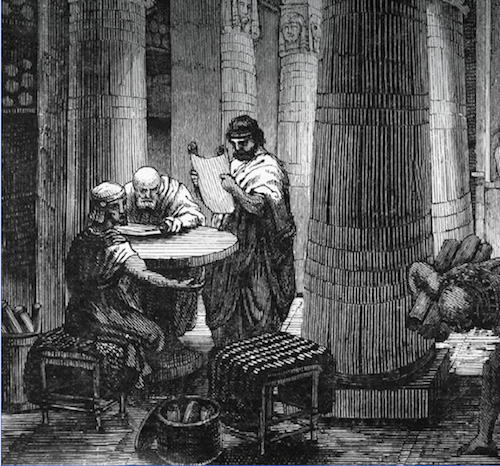
\includegraphics[width=1\textwidth]{figures/illustrasi.JPG}}
	\caption{ilustrasi yang tidak bertanggal dari para ilmuwan di Perpustakaan Alexandria © Bettmann / CORBIS}
	\label{illustrasi gambar}
	\end{figure}
\subsection(Bapak Geografi)
Eratosthenes melanjutkan pengetahuannya tentang Bumi. Dengan menggunakan penemuan dan pengetahuan tentang ukuran dan bentuknya, dia mulai membuat sketsa. Di Perpustakaan Alexandria ia memiliki akses ke berbagai buku perjalanan, yang berisi berbagai bentuk informasi dan representasi dunia. \cite{smith2005dictionary} Dalam karya jilid tiga-nya Geografi (bahasa Yunani: Geographika), dia menggambarkan dan memetakan seluruh dunia yang dikenalnya, bahkan membagi Bumi menjadi lima zona iklim: \cite{grimbly2013encyclopedia} dua zona pembekuan di sekitar kutub, dua zona beriklim sedang, dan sebuah zona yang meliputi khatulistiwa dan daerah tropis. Ia telah menemukan geografi. Dia menciptakan terminologi yang masih digunakan sampai sekarang. Dia meletakkan grid garis tumpang tindih di atas permukaan Bumi. Dia menggunakan kesejajaran dan garis meridian untuk menghubungkan setiap tempat di dunia. Sekarang mungkin untuk memperkirakan jarak seseorang dari lokasi dasar jaringan ini di atas permukaan Bumi. Dalam Geografi nama-nama lebih dari 400 kota dan lokasi mereka ditunjukkan: \cite{o1998eratosthenes} Sayangnya, Geografi-nya telah hilang dari sejarah, Pliny, Polybius, Strabo, dan Marcianus. \cite{roller2010eratosthenes}
Buku pertama adalah pengantar dan memberikan ulasan tentang pendahulunya, mengakui kontribusi mereka yang dia susun di perpustakaan. Dalam buku ini Eratosthenes mengecam Homer karena tidak memberikan wawasan tentang apa yang sekarang digambarkannya sebagai geografi. Ketidaksetujuannya terhadap topografi Homer membuat marah banyak orang yang percaya bahwa dunia digambarkan dalam Odyssey sebagai hal yang sah. \cite{eckerman2011eratosthenes} Bumi adalah dunia yang tak tergoyahkan; Sementara di permukaannya ada tempat yang sedang berubah. Dia telah berhipotesis bahwa pada suatu waktu Mediterania adalah danau besar yang menutupi negara-negara yang mengelilinginya; dan hanya terhubung ke barat saat sebuah lorong telah dibuka dalam sejarahnya.
Dalam buku kedua adalah penemuannya tentang keliling bumi. Di sinilah, menurut Pliny, "Dunia digenggam." Eratosthenes menggambarkan kisah terkenalnya tentang sumur di Syene, yang dijelaskan di atas. Buku ini akan dianggap sebagai teks tentang geografi matematika.
Buku ketiganya tentang Geografi berisi geografi politik. Dia mengutip negara-negara dan menggunakan garis sejajar untuk membagi peta menjadi beberapa bagian, untuk memberikan deskripsi alam yang akurat. Ini adalah terobosan, dan bisa dianggap sebagai awal geografi. \cite{smith2005dictionary}
\subsection(Mempelajari Bumi)
Eratosthenes mungkin orang pertama yang menggunakan kata geografi. Dia menciptakan sistem garis bujur dan garis lintang dan membuat peta dari dunia yang sekarang dikenal. Dia juga merancang sistem untuk menemukan penomoran utama — bilangan bulat yang hanya dapat dibagi sendiri atau dengan angka 1. Metode ini, masih digunakan sampai hari ini.
Pada saat itu, Eratosthenes mengusulkan sebuah algoritma sederhana untuk menemukan bilangan prima. Algoritma ini dikenal dalam matematika sebagai “Sieve of Eratosthenes.”
Dalam matematika, Sieve of Eratosthenes (Yunani: κόσκινον Ἐρατοσθένους), salah satu dari sejumlah saringan bilangan prima, adalah algoritma kuno yang sederhana untuk menemukan semua bilangan prima sampai batas tertentu. Hal itu terjadi karena secara iteratif menandai sebagai komposit, yaitu, tidak prima, kelipatan masing-masing prima, dimulai dengan kelipatan 2. Kelipatan bilangan prima yang diberikan dihasilkan mulai dari yang prima, sebagai urutan angka dengan perbedaan yang sama, sama dengan yang prima, antara angka berurutan. Ini adalah perbedaan kunci saringan dari penggunaan divisi percobaan untuk menguji secara berurutan setiap nomor kandidat untuk dibagi masing-masing prima.
Eeratosthenes juga yang pertama menghitung sumbu kemiringan bumi, yang dia pikir dengan tingkat akurasi yang tinggi; temuan dilaporkan oleh Ptolemy (85-165 M). Eratosthenes juga menghitung jarak dari bumi ke bulan dan ke matahari, tetapi dengan tingkat akurasi yang rendah. Ia membuat katalog 675 bintang. Ia membuat kalender dengan tahun kabisat dan meletakkan dasar chro- nology di dunia barat dengan penyelenggaraan tanggal sastra dan politik kegiatan dari pengepungan Troy (sekitar 1194 - 1184 SM) ke dalam waktu ia sendiri.
Namun, pencapaiannya yang paling abadi adalah perhitungan lingkar bumi yang sangat akurat (jarak di sekitar lingkaran atau bola). Dia menghitung ini dengan menggunakan geometri dan trigonometri sederhana dan dengan mengenali Bumi sebagai bola di ruang angkasa. Sebagian besar ilmuwan Yunani pada masa Aristoteles (384-322 SM) sepakat bahwa Bumi adalah sebuah bola, tapi tidak ada yang tahu seberapa besar itu.
Bagaimana para ilmuwan Yunani mengetahui bahwa bumi adalah sebuah lingkungan? Mereka mengamati bahwa kapal menghilang di atas cakrawala sementara tiang-tiang mereka masih terlihat. Mereka melihat bayangan melengkung Bumi di Bulan selama gerhana bulan. Dan mereka melihat perubahan posisi bintang di langit.
\begin{figure}[ht]
	\centerline{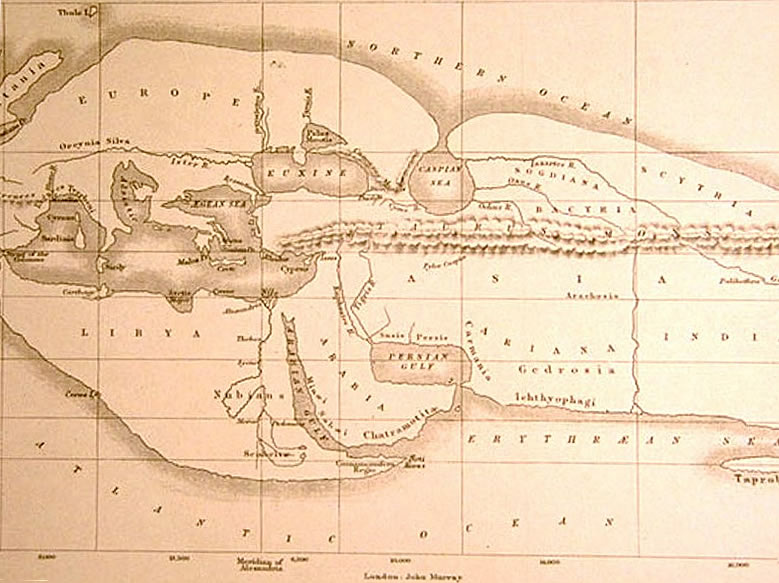
\includegraphics[width=1\textwidth]{figures/194BCE world map.JPG}}
	\caption{Rekonstruksi Eratosthenes c. 194 SM peta dunia, dari E.H. Bunbury's 1883 Sejarah Geografi Kuno di antara orang Yunani dan Romawi dari Abad Pertengahan sampai Kejatuhan Kekaisaran Romawi, ranah publik}
	\label{194BCE world map}
	\end{figure}
\subsection(Mengukur Bumi)
Eratosthenes mendengar tentang sumur terkenal di kota Swenet Mesir (Syene dalam bahasa Yunani, dan sekarang dikenal sebagai Aswan), di Sungai Nil. Siang hari satu hari setiap tahun - titik balik matahari musim panas (antara 20 Juni dan 22 Juni) - sinar matahari bersinar langsung ke dalam lubang dalam. Mereka hanya menyinari air di bagian bawah, bukan sisi sumur seperti pada hari-hari lain, membuktikan bahwa Matahari langsung di atas kepala. (Syene terletak sangat dekat dengan apa yang kita sebut Tropic of Cancer, ~ 23,5 derajat ke utara, garis lintang paling utara di mana Matahari selalu berada di atas kepala pada siang hari.)
Eratosthenes mendirikan sebuah tiang di Alexandria, dan pada titik balik matahari musim panas ia mengamati bahwa ia melemparkan bayangan, membuktikan bahwa Matahari tidak berada di atas kepala tetapi sedikit ke selatan. Mengakui kelengkungan Bumi dan mengetahui jarak antara kedua kota memungkinkan Eratosthenes untuk menghitung lingkar planet.
\cite{nicastro2008circumference} Eratosthenes bisa mengukur sudut sinar matahari dari vertikal dengan membagi panjang kaki di seberang sudut (panjang bayangan) dengan kaki yang bersebelahan dengan sudut (tinggi tiang). Ini memberinya sudut 7,16 derajat. Dia tahu bahwa lingkar bumi membentuk lingkaran 360 derajat, jadi 7,12 (atau 7,2, untuk membagi 360 secara merata sampai 50) derajatnya kira-kira seper lima puluh keliling. Dia juga tahu perkiraan jarak antara Alexandria dan Syene, jadi dia bisa mengatur persamaan ini:

Eratosthenes memperkirakan jarak dari Alexandria ke Syene sebanyak 5.000 stadion, atau sekitar 500 mil (800 kilometer). Dia membuat estimasi ini dari saat dibutuhkan pejalan kaki, yang dilatih untuk mengukur jarak dengan mengambil langkah reguler, untuk berjalan-jalan di antara kota-kota. Dengan memecahkan persamaan tersebut, dia menghitung keliling 250.000 stadia, atau 25.000 mil (40.000 kilometer) seperti pada gambar \ref{diagram pengukuran bumi}.
\begin{figure}[ht]
	\centerline{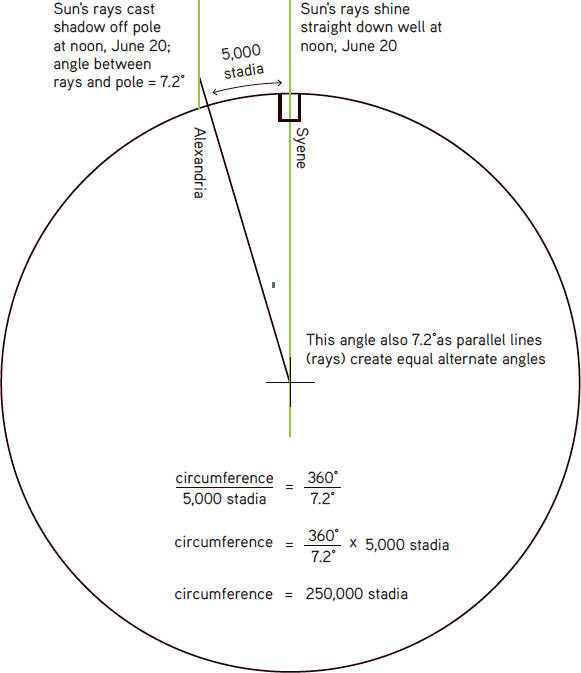
\includegraphics[width=1\textwidth]{figures/diagram pengukuran bumi.png}}
	\caption{Sebuah diagram yang menunjukkan bagaimana Eratosthenes mengukur Bumi, diakses dari Simon Fraser University Online}
	\label{diagram pengukuran bumi}
	\end{figure}
Beberapa sumber kesalahan merembet ke dalam perhitungan Eratosthenes dan interpretasi kita terhadapnya. Untuk satu hal, dia menggunakan unitnya untuk mengukur satuan "stadion" Yunani atau stadion atletik. Tapi tidak semua stadion dibangun dengan panjang yang sama. Di Yunani sebuah stadion setara dengan 185 meter (607 kaki), sedangkan di Mesir stadion berjarak sekitar 157,5 meter (517 kaki). Kami tidak tahu unit mana yang digunakan Eratosthenes. Jika dia menggunakan ukuran Yunani, perhitungannya akan turun sekitar 16 persen. Jika dia menggunakan orang Mesir, kesalahannya akan berada di bawah 2 persen dari lingkar bumi sebenarnya dari 24.860 mil (40.008 kilometer).
Satu abad setelah Eratosthenes, astronom Yunani Posidonius dari Rhodes (sekitar 135-51 SM) menghitung lingkar bumi. Posidonius menggunakan bintang Canopus sebagai kerangka acuan: ketika bintang tersebut terlihat di cakrawala di Rhodes, itu adalah 7,5 derajat di atas cakrawala di Alexandria. Perhitungan pertamanya hampir benar, tapi dia merevisi jarak antara Rhodes dan Alexandria, yang menghasilkan angka yang sebanding dengan sekitar 18.000 mil (sekitar 29.000 kilometer), sekitar 28 persen lebih kecil dari lingkar sebenarnya. Ptolemy melaporkan perhitungan Posidonius dan bukan kata-kata Eratosthenes, dan tulisan Ptolemy inilah yang menemukan jalan mereka menuju Christopher Columbus. Jika Ptolemy telah menggunakan sosok Eratosthenes yang lebih besar dan lebih akurat untuk keliling bumi, Columbus mungkin tidak akan pernah berlayar ke barat.
Eratosthenes hidup sampai usia 82 tahun, saat dia kelaparan sampai mati karena dia takut pada awitan kebutaan.
\subsection(Prestasi)
Eratosthenes digambarkan oleh Leksikon Suda sebagai Πένταθλος (Pentathlos) yang dapat diterjemahkan sebagai "All-Rounder", karena ia ahli dalam berbagai hal: Dia adalah seorang polymath sejati. Dia dijuluki Beta karena dia hebat dalam banyak hal dan mencoba mendapatkan setiap informasi, namun tidak pernah mencapai peringkat tertinggi dalam segala hal; Straboaccounts Eratosthenes sebagai matematikawan di antara ahli geografi dan ahli geografi di kalangan matematikawan.
• Eusebius dari Kaisarea dalam bukunya Preparatio Evangelica mencakup sebuah bab singkat dari tiga kalimat pada jarak selestial (Kitab XV, Bab 53). Dia menyatakan dengan sederhana bahwa Eratosthenes menemukan jarak ke Matahari untuk menjadi "σταδίων μυριάδας τετρακοσίας καὶ ὀκτωκισμυρίας" (secara harfiah "stadion miriad 400 dan 80.000") dan jarak ke Bulan menjadi 780.000 stadion. Ungkapan jarak ke Matahari telah diterjemahkan sebagai 4.080.000 stadia (1903 terjemahan oleh E. H. Gifford), atau sebagai 804.000.000 stadia (edisi Edouard des Places, bertanggal 1974-1991). Artinya tergantung pada apakah Eusebius berarti 400 segudang ditambah 80.000 atau "400 dan 80.000" segudang. Dengan stadion 185 m, 804.000.000 stadion adalah 149.000.000 km, kira-kira jaraknya dari Bumi ke Matahari.
• Menurut \cite{smith2005dictionary} Eratosthenes juga menghitung diameter Matahari. Menurut Macrobious, Eratosthenes membuat diameter Matahari menjadi sekitar 27 kali lipat dari Bumi. Angka sebenarnya kira-kira 109 kali.
• Selama berada di Perpustakaan Alexandria, Eratosthenes merancang sebuah kalender dengan menggunakan ramalannya tentang ekliptika Bumi. Dia menghitung bahwa ada 365 hari dalam setahun dan setiap tahun keempat akan ada 366 hari.
• Dia juga sangat bangga dengan solusinya untuk Menggandakan Cube. Motivanya adalah bahwa ia ingin menghasilkan ketapel. Eratosthenes membangun perangkat gambar garis mekanis untuk menghitung kubus, yang disebut mesolabio. Dia mendedikasikan solusinya untuk Raja Ptolemy, menyajikan sebuah model di perunggu dengan sebuah surat dan sebuah epigram. Archimedes adalah teman Eratosthenes dan dia juga mengerjakan alat perang dengan matematika. Archimedes mendedikasikan bukunya The Method to Eratosthenes, mengetahui cintanya untuk belajar dan matematika. \cite{chondros2010archimedes}
\subsection(Pekerjaan)
Eratosthenes adalah salah satu tokoh ilmiah paling terkemuka di masanya, dan menghasilkan karya-karya yang mencakup pengetahuan luas sebelum dan selama waktunya di Perpustakaan. Dia menulis banyak topik - geografi, matematika, filsafat, kronologi, kritik sastra, tatabahasa, puisi, dan bahkan komedi lama. Sayangnya, hanya ada sisa fragmen karya-karyanya setelah Penghancuran Perpustakaan Alexandria.
\subsection(Gelar)
1.	Platonikos
2.	Hermes
3.	Erigone
4.	Chronographies
5.	Pemenang Olimpiade
6.	\cite{thomasselections} Περὶ τῆς ἀναμετρήσεως τῆς γῆς (Pada Pengukuran Bumi) (hilang, diringkas oleh Cleomedes)
7.	Гεωγραφικά (Geographika) (hilang, dikritik oleh Strabo)
8.	Arsinoe (sebuah memoar Ratu Arsinoe; hilang; \cite{gulickathenaeus})
9.	\cite{gulickathenaeus} Ariston (tentang Aristo dari Chios 'kecanduan kemewahan); kalah; dikutip oleh Athenaeus di Deipnosophistae)
10.	Koleksi fragmen mitos Helenistik tentang rasi bintang, yang disebut Catasterismi (Katasterismoi), dikaitkan dengan Eratosthenes, mungkin untuk menambah kredibilitasnya.
>>>>>>> b69ba4276178623acc4d88cec883f12776ed0ed0
